The following chapter elaborates on the methods and techniques used to compare the returns of applying deep learning algorithms to small cap- and large cap stock predictions. It presents a variety of deep learning models used for predicting returns for both large cap and small cap stocks on the Oslo Stock Exchange. The aim of the research is to evaluate if the excess returns of investing in small caps can be capitalized on, through deep learning algorithms being able to detect patterns and relationships within historical data and by making accurate predictions of the probability of future share price development. An important part of a research process is choosing the appropriate method and research design to correctly analyze information and data on the topic, as well as for others to be able to assess the reliability and validity of the paper. 

\indent\newline
The methodology and techniques used in this paper is inspired by the work of Krauss et al. and Lund et al. \cite{krauss} \cite{lund}. This means that a similar approach and framework for developing the algorithms and assessing the models' predictive performance is applied to predicting small cap stock returns. In addition to exploring the models' applicability to small cap stock returns, the paper will add on previous work in terms of implementing a gated recurrent unit (GRU) and a convolutional neural network (CNN).   

\indent\newline
The methodology can be decomposed into five sections, where the first three presents how the networks are trained and tested, how the dependent variable is created, the different independent features that are included, and the networks' hyperparameters. Further, an explanation of how the models' predictive performance are evaluated is presented, before defining different trading strategies and their applicability to a real-life trading scheme.  

\section{Long Short-Term Memory Network}

\subsection{Training and Testing}
The process of training the algorithms starts by defining a study period based on the collected data set, which contains data from January 1st 2005 to December 31st 2020. This involves splitting the data into a training set and a test set. The training set has an interval of 750 trading days, while the test set has an interval of 250 trading days. Given that stock markets are closed on the weekend and during holidays, 750 trading days translates into approximately 3 years while 250 trading days translates into 1 year. The training period is where the LSTM-network learns the patterns within the data and adjusts parameters to increase predictive accuracy, while the trading sets (test sets) are used to make out-of-sample predictions. The study periods are divided into a total of 23 unique periods, where each period is set up as rolling blocks of 1000 days. This means that the first period of trading (testing) starts 750 days into the data set, where these first days are lost to training. Further, each study period begins 250 days after the previous one, to ensure that the trading periods are non-overlapping, which means testing the models' predictions on the same data is avoided \cite{krauss}. 
\indent\newline 
\begin{figure}[H]
\centering
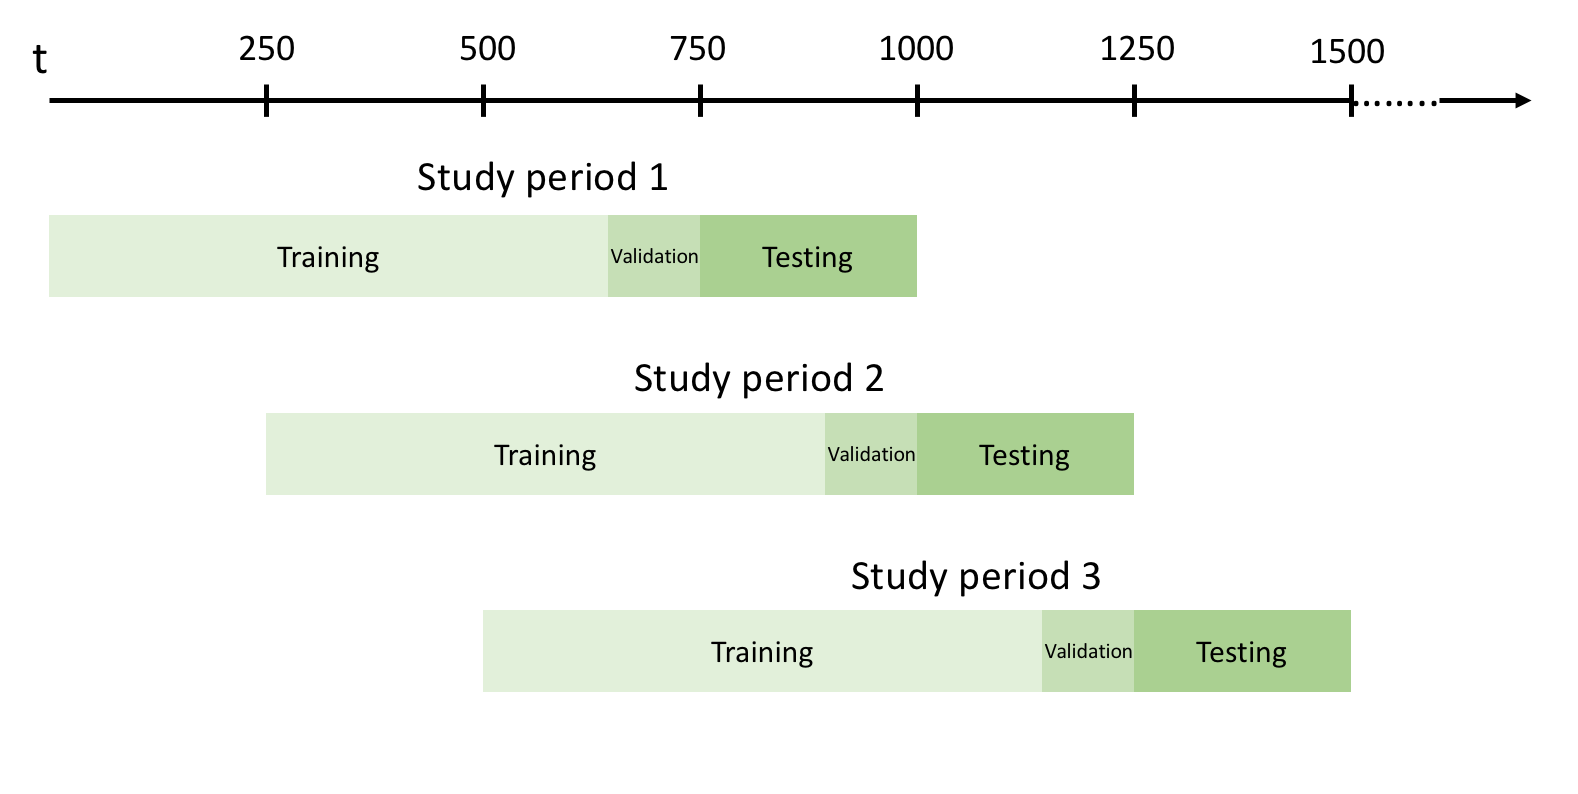
\includegraphics [scale=0.48,angle=360]{figures/study.png}
\caption{Rolling Study Periods}
\label{fig:study}
\end{figure}

\indent\newline 
Figure 4.1 illustrates the logical reasoning behind the study periods, where the last 20\% of the training data is used for validation. Including validation sets is important in order to avoid selection bias related to the process of hyperparameters-optimization.

\indent\newline
The training and testing sequences are applied to two different groups of stocks, where one is a group consisting of small cap stocks that are constituents of the OSESX small cap index and the other is a group of large cap stocks that are constituents of the OSEBX benchmark index. For both groups, $n_{i}$ denotes the number of stocks that are part of indices at the last day in study period $\textit{i}$. Some of the stocks may not have a full data history for each training period, due to either delisting, being listed at a later time, or implemented in another index. If stocks do not exhibit share price data after a certain point in the trading period, they are included for trading up until this point.     

\subsection{Independent Variables}
In order to improve model performance in terms of finding patterns and relationships within the data, several independent variables are used as input features for the models to train and test on. According to previous research, including a standardized one-day return with a sequence length of 240 days as a main independent variable seems to give good results with this type of neural network \cite{krauss}. To create the feature, the price process of stock $\textit{s}$ at time $\textit{t}$ is defined as $P^{s}$ = $(P^{s}_{t})_{t\in T}$ and where the simple return $R^{m,s}_{t}$ for a stock $\textit{s}$ over $\textit{m}$ periods is calculated in the following way:

\indent\newline
$R^{m,s}_{t}$ = $\frac{P^{s}_{t}}{P^{s}_{t-m}}$ - 1

\indent\newline
The simple returns are calculated for each day and each stock $R^{1,s}_{t}$. Further, the mean and standard deviation are obtained from the training set. It is important to compute these measures only from the training set, as it ensures the network to avoid look-ahead biases. The mean $\mu^m_{train}$ is then subtracted from the simple returns and divided by the standard deviation $\sigma^{m}_{train}$ to standardize the returns:

\indent\newline
$\tilde{R}^{m,s}_{t}$ = $\frac{R^{m,s}_{t} - \mu^m_{train}}{\sigma^{m}_{train}}$

\indent\newline
The training process of an LSTM network requires input features to be divided into different sequences. As mentioned earlier, the standardized one-day returns $\tilde{R}^{1,s}_{t}$ have a sequence length of 240 days, which translates into approximately one year of trading. The standardized one-day returns are organized in overlapping sequences, where the feature vector is sorted by stocks $\textit{s}$ and date $\textit{t}$ in ascending order. To illustrate this, the first two sequences of the first stock $s_{1}$ have the form of $\lbrace\tilde{R}^{1,s_{1}}_{1}, \tilde{R}^{1,s_{1}}_{2}, ..., \tilde{R}^{1,s_{1}}_{240}\rbrace$ and $\lbrace\tilde{R}^{1,s_{1}}_{2}, \tilde{R}^{1,s_{1}}_{3}, ..., \tilde{R}^{1,s_{1}}_{241}\rbrace$ and so forth \cite{krauss}. 
   

\indent\newline
A large segment in the Norwegian economy is based on oil-related companies and represents a substantial part of the Oslo Stock Exchange's total market cap. Brent-oil price is therefore regarded as an important influence on the Oslo Stock Exchange and will be included as an input feature. Other independent variables that represent macroeconomic factors are the USD/NOK exchange rate and the 10-year US treasury rate, which are also included as input features. Additional input features are based on technical indicators and consist of the stock's daily volume, and moving averages with intervals of 50 and 200 days. Lastly, a measure of the broad market volatility is included as an input feature through daily data on the CBOE Volatility Index (VIX), also known as the fear index. The VIX captures market sentiment by measuring the relative strength of near-term price changes of the S\&P 500. It generates a 30-day forward projection of volatility, by being derived from prices of SPX index options with near-term expiration dates \cite{kuepper2021}.


\indent\newline
The reasoning behind including the 10-year US treasury rate and the VIX is their influence on small cap stocks. A majority of small cap stocks are not expected to generate positive cash flow before several years down the line. When investors calculate the net present value (NPV) of these companies, the rate of US treasuries affects the discount rate included in their NPV-analysis. 

\indent\newline
NPV = $\sum_{t=1}^{n} \frac{R_{t}}{(1 + i)^{t}}$

\indent\newline
The equation above shows the formula for calculating the NPV, where $R_{t}$ is the expected net cash flow in a single time period $\textit{t}$, $\textit{i}$ is the discount rate which is based on potential returns from alternative investments, and $\textit{t}$ is the number of time periods. When investors decide on which discount rate to include in their analysis, they evaluate other returns from alternative investments. The 10-year treasury yield is a measure of a risk free rate and an alternative investment, and therefore affects the discount rate. E.g. if the risk free rate goes up, the discount rate also goes up and vice versa. A higher discount rate means that the present value of (especially) small cap stocks' future positive cash flow is negatively affected, since the positive cash flows are not expected until several years into the future. The 10-year US treasury rate should therefore, to a certain degree, explain the variability in small cap stocks' share price. Small cap stocks also tend to be more volatile than large cap stocks, which give reason to believe that the VIX could be a suitable input feature to include when predicting small cap stock returns. 

\subsection{Target Variable}
Following Krauss et al. the target variable $Y^{s}_{t + 1}$ represents a binary classification problem with two classes. The dependent variable for each stock $\textit{s}$ and date $\textit{t}$ is therefore equal to a value of either 1 or 0. This is determined on the basis of whether the one-period return $R^{1,s}_{t + 1}$ of stock $\textit{s}$ is larger or equal (class 1) to the cross-sectional median return of all stocks in period $\textit{t + 1}$, or smaller (class 0) than the cross-sectional median return. The classes are defined by ordering all one-period returns $R^{1,s}_{t + 1}$ of all stocks $\textit{s}$ in period $\textit{t + 1}$ in ascending order, and by putting them into two equally sized classes \cite{krauss}.   


\subsection{Hyperparameters}

\section{Gated Recurrent Unit Network}

\subsection{Training and Testing}

\subsection{Independent Variables}

\subsection{Target Variable}

\subsection{Hyperparameters}

\section{Convolutional Neural Network}

\subsection{Training and Testing}

\subsection{Independent Variables}

\subsection{Target Variable}

\subsection{Hyperparameters}

\section{Evaluation Metrics}
\subsection{Predictions}
Several threshold metrics for classification are used to assess and evaluate the accuracy of the networks. The section presents five performance metrics chosen on the basis of quantifying the prediction errors and accuracy of the networks, either by a fraction, ratio or rate. The first metric measures the networks' accuracy, which is the fraction of observations correctly classified:

\indent\newline
$Accuracy = \frac{CP}{TP}$

\indent \newline 
\textit{Where,
\begin{itemize}
    \item[] $CP$ = Correct predictions
    \item[] $TP$ = Total predictions
\end{itemize}
}

\indent \newline 
The next metric is quite similar to the previous one, but instead of measuring the amount of correct predictions compared to total predictions, it compares the amount of positive/negative predictions with total positive/negative predictions:

\indent\newline
$PA = \frac{CPP}{TPP}$

\indent \newline 
\textit{Where,
\begin{itemize}
	\item[] $PA$ = Positive accuracy
    \item[] $CPP$ = Correct positive predictions
    \item[] $TPP$ = Total positive predictions
\end{itemize}
}

\indent \newline 
Another metric incorporated to evaluate network performance is recall. The measurement looks at the ratio of the networks’ correct positive prediction compared to the amount of actual positive observations:

\indent\newline
$Recall = \frac{CPP}{TPO}$

\indent \newline 
\textit{Where,
\begin{itemize}
    \item[] $CPP$ = Correct positive predictions
    \item[] $TPO$ = Total positive observations
\end{itemize}
}

\indent \newline 
The next metric is the F-score. It uses the positive accuracy and recall to measure the networks' predictive accuracy in terms of robustness:

\indent\newline
$F-Score = \frac{PA * Recall}{PA + Recall}$

\indent \newline 
\textit{Where,
\begin{itemize}
    \item[] $PA$ = Positive accuracy
\end{itemize}
}

\indent \newline 
The fifth and last evaluation metric is binary cross-entropy, which is the networks' loss function during training. In addition to measuring if predictions are correct or not, it also takes into account the difference between the predicted probabilities and actual outcomes \cite{lund}:

\indent \newline 
$BCE = \frac{1}{N} \sum^{N}_{n=0} (y_{n}log[p_{n}] + (1 - y_{n})log[1 - p_{n}])$

\indent \newline 
\textit{Where,
\begin{itemize}
    \item[] $BCE$ = Binary cross entropy
    \item[] $N$ = Number of observations
    \item[] $y_{n}$ = Actual class of observation n
    \item[] $p_{n}$ = Predicted probability of observation n    
\end{itemize}
}

\subsection{Trading}

\section{Strategies}

\section{Predictive Models }
\subsection{ Benchmark Algorithms}
Random forest is a classification algorithm which consists of a large number of individual decision trees that works like an ensemble. Decision trees split the data into branches, or subsets, where certain learning conditions enable the algorithm to classify observations. Random forest operates like an ensemble since it uses multiple algorithms to improve the performance and accuracy of the predictions. In a binary case, each individual tree performs a class prediction, where the class with most predictions is selected as the model's prediction. Combining several decision trees reduces the probability of overfitting and situations where the model finds optimal solutions that are local instead of global. Logistic regression is another algorithm used for classification problems. It resembles linear regression, but uses a more complex cost function known as the Sigmoid function to return a probability value \cite{pant}. 

\subsection{Deep Learning Algorithms}
The deep learning algorithms which will be used in the paper will consist of variations of neural networks that are based on both a feedforward architecture and recurrent architecture. Feedforward neural networks are regarded as simpler than recurrent neural networks since the information only moves forwards and not backwards through the network. In contrast, recurrent neural networks have connections between nodes characterized as a directed graph, which forms a cycle. The network is thus able to retain its state while processing the next sequence of inputs. Current suggestions for algorithms to be incorporated in the paper consist of simple recurrent neural networks (SRNN), gated recurrent units (GRU), and long short-term memory networks (LSTM). LSTM is a type of recurrent neural network and consists of cells, input and output gates, and a forget gate, which makes the algorithm well-suited for financial time series. GRU is also a form of recurrent neural network that possesses similar traits as LSTM. However, the algorithm does not have an output gate and therefore has fewer parameters than LSTM. Previous evidence suggests that the algorithm is suitable for smaller and less frequent data sets \cite{jun}.   
   